\documentclass[titlepage]{article}

\usepackage[margin=1in]{geometry}
% some more shit for the title
\usepackage[T1]{fontenc}
\usepackage{babel}

% Tables and stopping them from displaying in a different section
\usepackage{booktabs}
\usepackage[section]{placeins}

% for inserting images into the document, setting file path, and allowing rotation of inserted images 
\usepackage{graphicx}
\graphicspath{ {./images/} }
\usepackage{rotating}
\usepackage[table]{xcolor}
% mostly just for putting text in math equations
\usepackage{amsmath}
% for aligning the text to the left
\usepackage[document]{ragged2e}

% for inserting hyperlinks in the document, use \url{url} or \href{url}{text}
\usepackage{hyperref}
\usepackage{calligra}
\usepackage[T1]{fontenc}
\usepackage{siunitx}
\usepackage{caption}
\usepackage{multirow}
\usepackage[export]{adjustbox}
\usepackage{tikz}
\usepackage{pgfplots}
\pgfplotsset{soldot/.style={color=black,only marks,mark=*},
	             holdot/.style={color=black,fill=white,only marks,mark=*},
		                  compat=1.12}
\usepackage{paracol}

\begin{document}
\title{\textbf{Lab 3: Capacitors in Series and Parallel}}
\author{
    Zachary Pouska\\
    \texttt{001103193}\\
    \and
    Natalie Tran \\ 
    \texttt{000698629}\\ \\
} 

\date{PHYS 236 | Fall 2022\\
Date performed: 09/28/2022}


	\maketitle



	\section{Purpose}
    The purpose of this lab is to gain a working understanding of the real-world behavior of capacitors, and experimentally finding the equivalent capacitance of various combinations of series and parallel capacitors.

	\section{Theory}	

    The following formula for percent difference was used throughout the lab: $$\text{\% difference} = \frac{|C_{eq}\text{measured} - C_{eq}\text{calculated} |}{\frac{1}{2} |C_{eq}\text{measured} + C_{eq}\text{calculated}|} \times 100$$



	\section{Experiment Analysis}
    



	\section{Procedure}

        \subsection{Measurement of Capacitance Using a Multi-Meter}
        Not using the breadboard to hold the capacitors in place, our group measured the capacitance of each capacitor while laying on the table. We then proceeded to fill out the values and calculate the percent errors in table 5.1.

        \subsection{Measurement of Equivalent Capacitance in Series}
        Beginning by assembling the capacitor circuit with backwards polarity to the example photo, our group proceeded to calculate and measure the values in table 5.2.\\ 


        \subsection{Measurement of Equivalent Capacitance in Parallel}
        After assembling the capacitors in parallel as shown in the figure below, our group collected the equivalent capacitance and calculated the percent difference shown in table 5.3.
        \begin{figure}[hbt!] 
            \centering
            \caption*{Part 2 Circuit Diagram}
            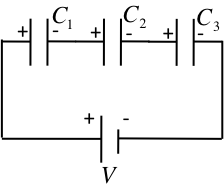
\includegraphics{images/procedure/part2.png}
        \end{figure} 




        \subsection{Measurement of Equivalent Capacitance for Both Series and Parallel}



	\section{Data and Graphs}
	    \subsection{Part 1}


	    \subsection{Part 2} 


	    \subsection{Part 3}

    \section{Calculations and Results}

        \subsection{Part 1} 

        \subsection{Part 2} 
        Zach

        \subsection{Part 3} 
        Zach

        \subsection{Part 4} 
        \subsection{Part 5} 
        \subsection{Part 6} 


	\section{Questions}


    	\subsection{Circuit 1}

        \begin{figure}[hbt!]
            \centering
            \caption{Circuit diagram for question 1}
            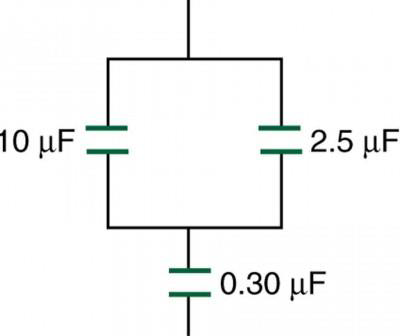
\includegraphics{questions/1}
        \end{figure}



    
    	\subsection{Circuit 2}
        \begin{figure}[hbt!]
            \centering
            \caption{Circuit diagram for question 2}
            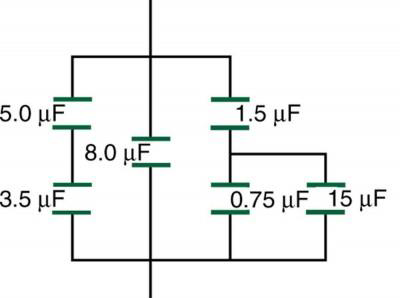
\includegraphics{questions/2}
        \end{figure}

    {{Calculations for finding $\mathbf{C_{eq}}$}}
        $$\left( \frac{1}{0.75\mu F+15\mu F}+\frac{1}{1.5\mu F} \right)^{-1}+\left(\frac{1}{3.5\mu F}+\frac{1}{5\mu F}\right)^{-1}+8\mu F  = 11.4 \mu F$$


    
    
  	\section{Conclusion}
    This was a very quick and informative lab. Our group was able to verify our calculations with very low percent differences, aside from the capacitors initially being quite off from their rated capacitances. 

\end{document}
